%------------------------------------------------
\begin{frame}
\frametitle{Sitting right}
\hypertarget{posture_sitting}{}
\begin{columns}[c] % The "c" option specifies centered vertical alignment while the "t" option is used for top vertical alignment

\column{.3\textwidth} % Left column and width

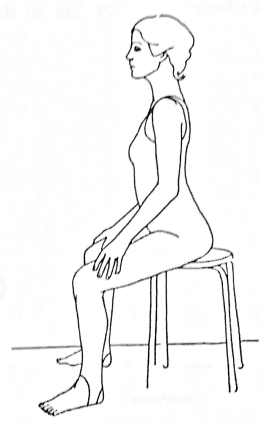
\includegraphics[width=\linewidth]{Sitting_posture}

\column{.7\textwidth} % Left column and width
Sit on the \structure{front third of the seat}, \structure{open your legs} to about the width of your body. 

The soles of both your feet have \structure{contact with the body}. The point of your tows and your knees point slightly out. 

Your \structure{calves and thighs} have a \structure{right angle} with each other. 

Give a slight \structure{pressure} with the knuckles of your ischium \structure{down} onto the surface of the seat and imagine how the \structure{chair pushes upwards} with the same force upwards. That will automatically make you hold your upper body in an upright position.
\end{columns}

\end{frame}
%------------------------------------------------
%------------------------------------------------
\begin{frame}
\frametitle{Sitting normal posture}

\begin{columns}[c] % The "c" option specifies centered vertical alignment while the "t" option is used for top vertical alignment

\column{.4\textwidth} % Left column and width

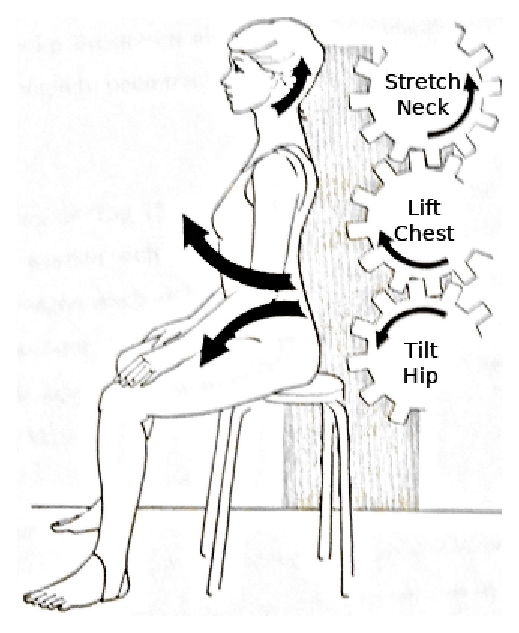
\includegraphics[width=\linewidth]{phys_posture}

\column{.6\textwidth} % Left column and width
This is the \structure{normal posture}, where the chest and the belly cavity give the inner \structure{organs enough space} and in which the \structure{spine} can fulfil its carrying function and act as the \structure{central axis}. 

When the body gets straightened up while seating, it will automatically \structure{tilt the hip forward}, the \structure{chest gets lifted} and the \structure{cervical spine stretched}. At the same time, the shoulder girdle will be placed in the right place.
\note{If somebody lets themselves fall into a \structure{bend posture}, the \structure{chest sinks}, the \structure{hip rolls back} and the \structure{shoulder girdle moves forward}. That makes the \structure{cervical spine} have a \structure{concave curvature}.}
\end{columns}

\end{frame}
%------------------------------------------------
